\rhead{Course Objectives}

\chapter{Course Objectives}

\begin{figure}[!h]
\centering
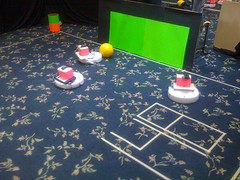
\includegraphics[width=0.8\columnwidth]{figures/1_teaser.jpg}
\end{figure}

\newpage

\begin{wrapfigure}{r}{0.35\columnwidth}
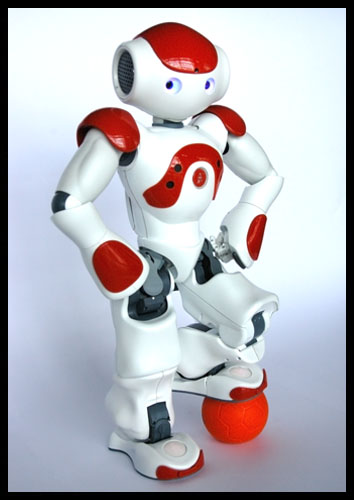
\includegraphics[width=0.3\columnwidth]{figures/1_Nao.jpg}
\caption{The Aldebaran Nao.}
\label{fig:1_Nao}
\end{wrapfigure}

This book is based on our experiences developing and restructuring an undergraduate robotics course, Brown University CS 148 ``Building Intelligent Robots'', for the iRobot Create platform.  Taking the perspective of CS 148, we describe our objectives and approach for an upper-level course in autonomous robotics.  Our main educational goal is to focus on the computational aspects of robotics while minimizing the necessary mechatronic startup costs, which is best suited for a complementary course.  To this end, we use a solderless robot platform comprised of ``off-the-shelf'' components that can be readily assembled by undergraduate (and secondary) students.  This platform is meant to be both a quick entry point for students to start programming robots and, using research-grade robot middleware (e.g., Player, ROS), a path that can directly lead to understanding and extending the state-of-the-art in robotics.

For instructors, this book is meant to be a ``how-to'' guide for getting an autonomous robotics course modules up-and-running with as little overhead as possible.  The first three chapters describe how to assemble, program and remotely control a basic low-cost mobile robot platform.  Subsequent chapters cover project modules suitable for this (and similar) mobile robotics, as conducted in CS 148 in recent years.  These projects build upon each other from bug and random navigation algorithms and color object recognition up through path planning, robot localization, subsumption architectures, multi-robot coordination, learning from demonstration, and experimentation with significance testing.  These projects are pedagogically cast within a ``robot control loop'' (consisting of sensing, perception, decision making, motion control, and physics).  The control loop serves as a conceptual scaffold similar to the notion of a pipeline in computer graphics. 

In terms of collaboration, this book is intended to be a community resource that facilitates sharing and collaboration in and beyond the classroom.  Given the larger integrative nature of robotics projects, CS 148 projects utilize version control systems (Subversion in particular) to enable collaboration among student groups, reproducibility by course graders, and portability when moving code across robots.  For educators, this book itself and supporting materials will be maintained (and continually updated) in a Subversion repository:

\begin{verbatim}
   http://brown-rlab.googlecode.com/svn/trunk/teaching_autonomous_robotics
\end{verbatim}

We encourage educators to freely use the book and materials in their courses and broader educational efforts.  These materials are meant to be copy-pasted, modified, tested, and refined as a community to improve the quality and accessibility of robotics education.  We welcome and encourage contributions to the continued development of this book, especially those that can be patched into the repository.  Up-to-date usage of these materials in CS 148 can be accessed through the course website:

\begin{verbatim}
   http://www.cs.brown.edu/courses/cs148
\end{verbatim}



\section{CS 148 Course Description}

\texttt{(taken from Brown 2009-10 course catalog)}

CS148 is an introduction to fundamental topics in autonomous robot control. This course focuses on the development of ``brains'' for robots. That is, given a machine with sensing, actuation, and computation, how do we develop programs that allow the machine to function autonomously? We answer this question through a series of class discussions and group projects.

CS148 class meetings cover technical and algorithmic aspects of robotic decision making and perception, as well as societal and philosophical implications posed by autonomous robots. Discussions amongst the class pose and address questions related to how robots can contribute to society, what technical functionality is needed, and how will such technologies affect the human-robot dynamic.

CS148 projects center on a ``robot soccer'' task, where students program robot vacuum-like devices to play soccer in a structured environment. Various approaches to robot control (spanning reaction to deliberation) are covered using the \href{http://robotics.cs.brown.edu/projects/smurv/}{Brown iRobot Create platform robots} (which are \href{http://www.irobot.com/sp.cfm?pageid=122}{iRobot Roomba/Create} hardware with onboard ASUS EeePC subnotebooks, as seen in Figure \ref{fig:1_create_platform} on the far right). We support either the \href{http://playerstage.sourceforge.net}{Player/Stage/Gazebo (PSG)} robot framework or the \href{http://www.ros.org/wiki/ROS/StartGuide}{Robot Operating System (ROS)} as a robot middleware solution for the course projects. Similarly, the project implementations are not restricted to the iRobot Create platforms. Rather any robot that has the physical components for playing soccer, such as Aldebaran's \href{http://www.aldebaran-robotics.com/eng/Nao.php}{Nao humanoid robot} (Figure \ref{fig:1_Nao}), can be used to program the assignments. Thus, the practical aspects of this course are not limited to a specific robot platform or middleware. 

\begin{figure}[!h]
\centerline{
\mbox{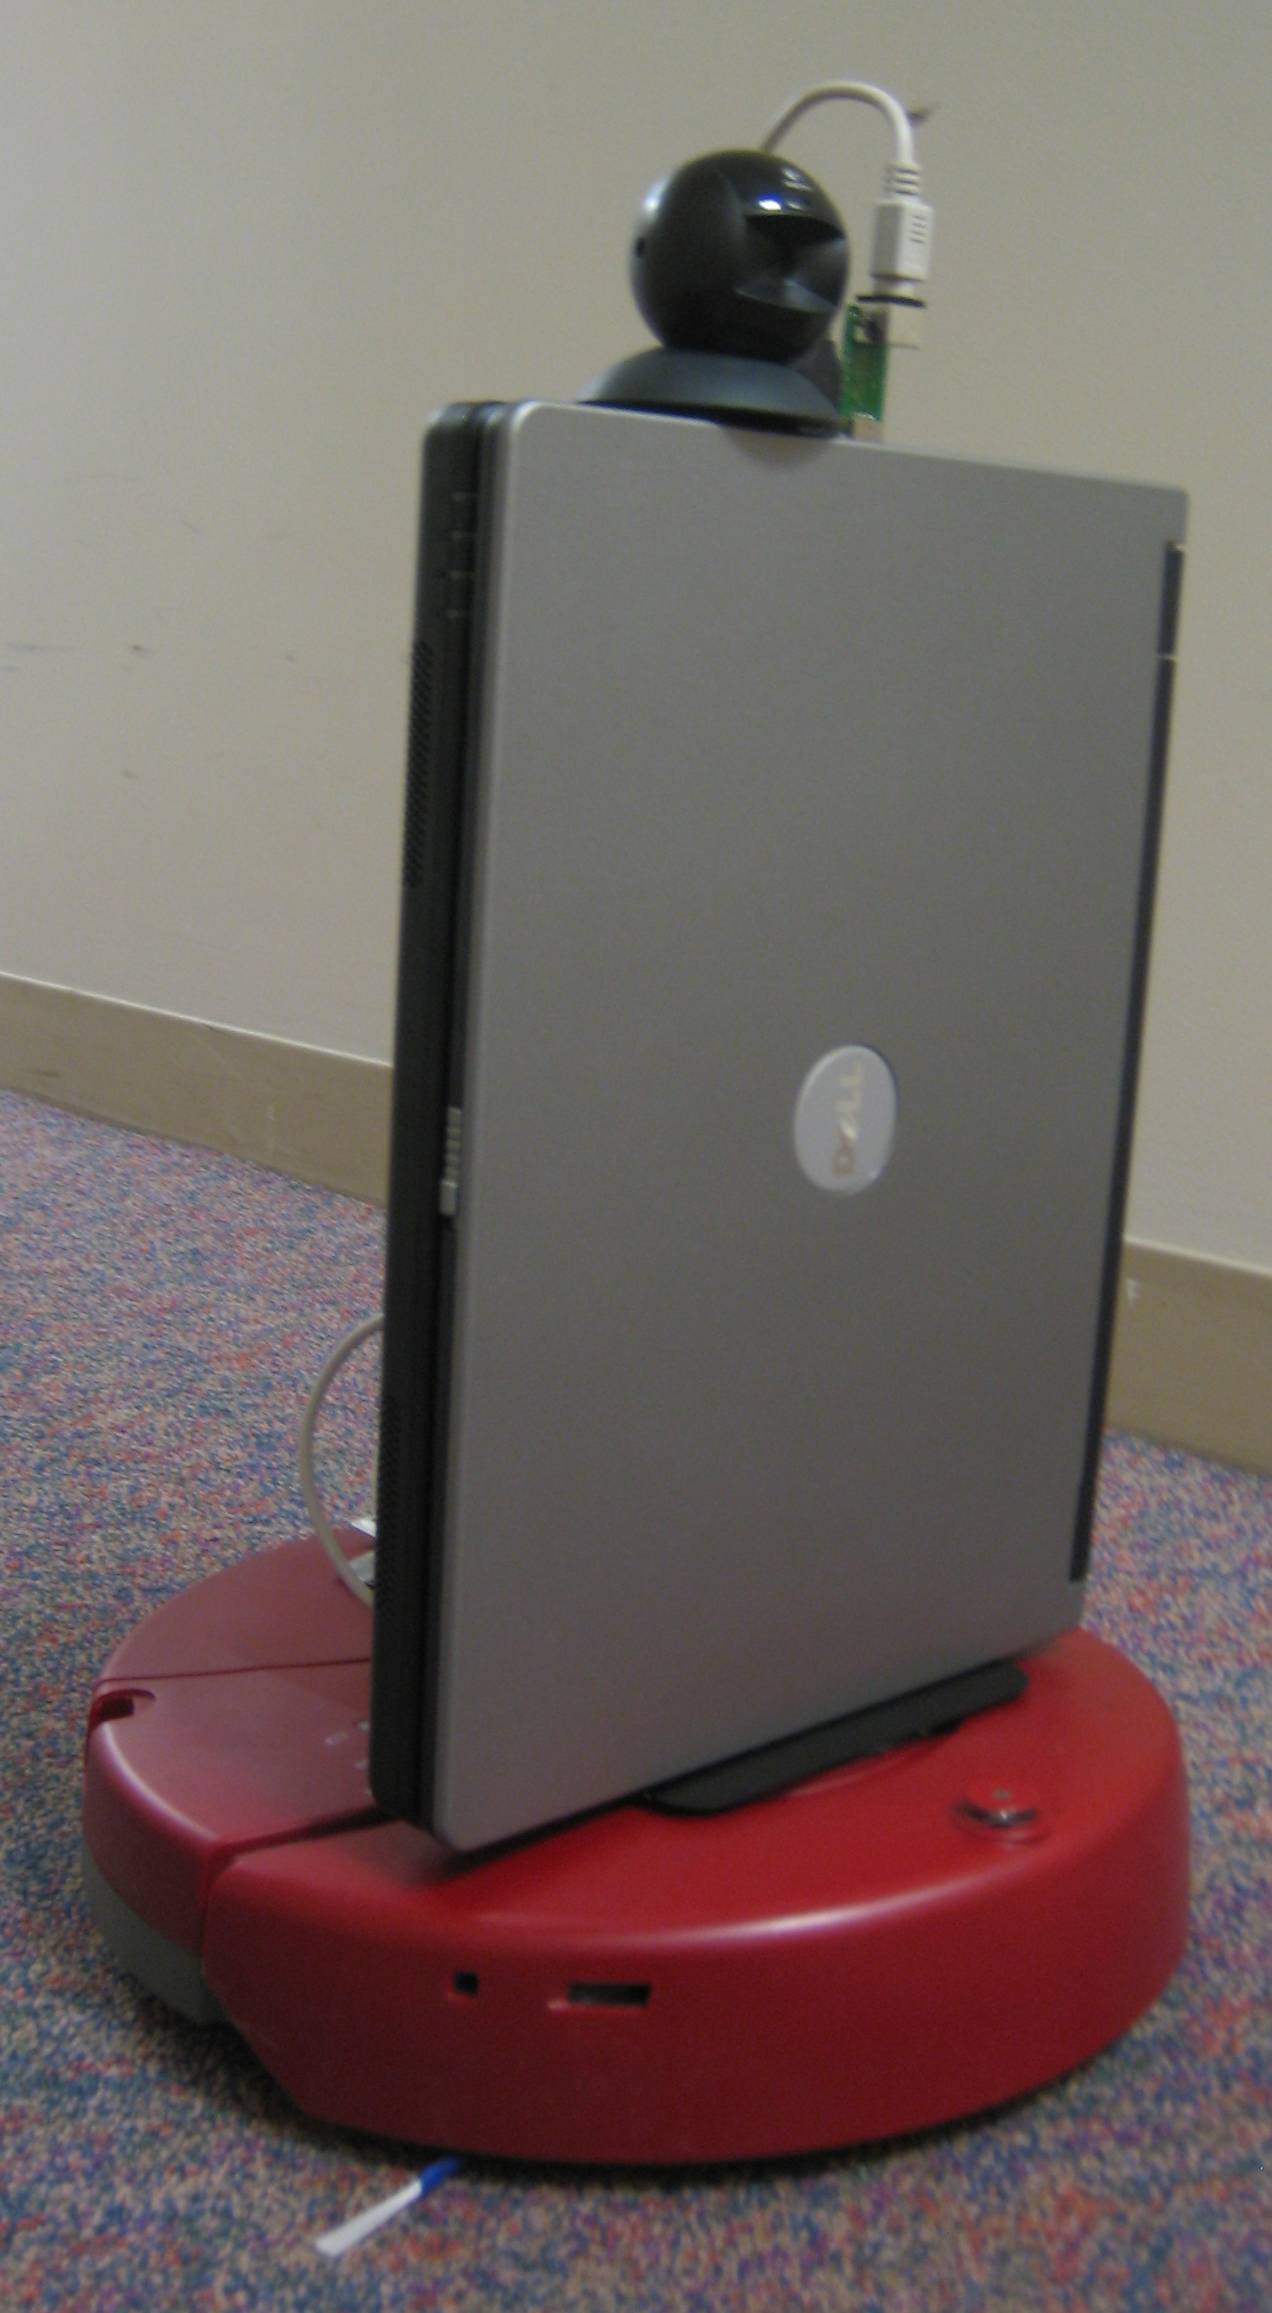
\includegraphics[height=1.6in]{figures/1_platformv1.png}}
\mbox{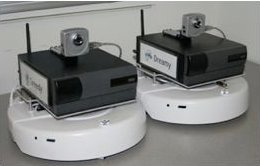
\includegraphics[height=1.6in]{figures/1_create_platformv1.jpg}}
\mbox{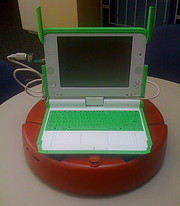
\includegraphics[height=1.6in]{figures/1_create_v2.jpg}}
\mbox{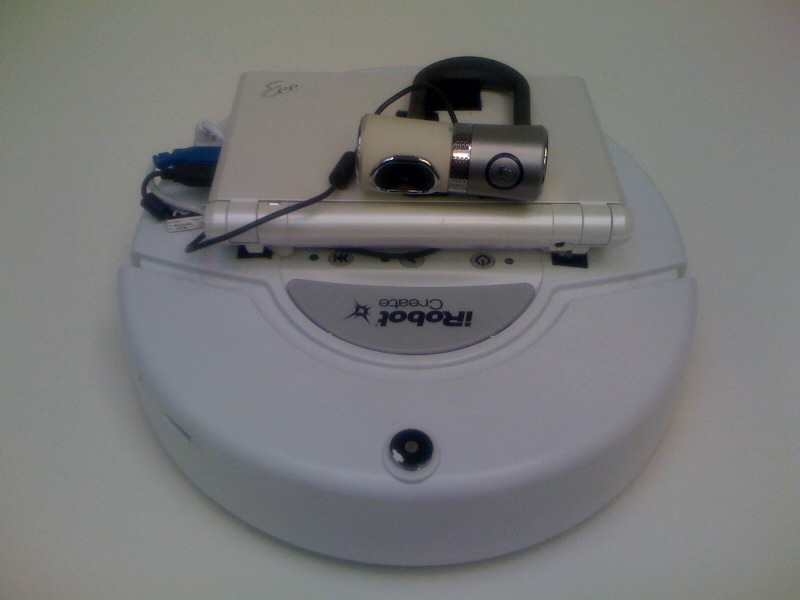
\includegraphics[height=1.6in]{figures/1_create_platform.jpg}}
}
\caption{Evolution of the Brown SmURV robot platform. Version 0.5 (2006), Logitech QuickCam and iRobot Roomba connected to a larger Dell laptop, usually carried offboard, using a RoboDynamics RooStick.  Version 1.0 (2007), a Mini-ITX computer and Unibrain Fire-I camera connected to and powered by an iRobot Create.  Version 1.5 (2008), a One Laptop Per Child XO, with onboard camera, connected to a Roomba.  Version 2.0 (2009), an Asus EEE PC and Logitech QuickCam Ultra on an iRobot Create. }
\label{fig:1_create_platform}
\end{figure}

%%\bkorel{picture of PS3 cam with newer laptop and create?)

\section{Why Robotics?}

Why should anyone consider robotics?  One quick answer: the 3 D's, ``Dirty, Dull, and Dangerous.''  Robots have long been proposed as a way to relieve humans from tasks necessary for society that can be unpleasant, mundane, or hazardous to human health.  More generally, robotics can be considered a means to enhance physical human productivity that augments or even multiplies a human user's ability to perform tasks in the physical world.

The application of robots already has a strong presence in many different fields, illustrated in the collage of Figure \ref{fig:1_robotic_applications}.  In healthcare, robots have assisted doctors, nurses, and caretakers in the delivery of medicines in hospitals, surgical operations, and post-stroke rehabilitation.  The use of robotics has the potential to reduce health care costs and help the elderly and chronically ill to remain independent. Exploration robots have been able to collect scientific data on planets and deep sea areas that would be difficult (perhaps impossible) for humans to reach.  Domestic service robots such as the iRobot Roomba and Willow Garage's PR2 can perform basic household chores, such as vacuuming and laundry.  Robots in manufacturing assist with labor intensive jobs to lower production costs and increase productivity.  Unmanned vehicles for military applications, such as the General Atomics MQ-1 Predator and iRobot PackBot, can provide greater reconnaissance and reduce the risk of human casualties by using robots in place of humans.  Along with the benefits of each of these applications, robots raise serious questions about unintended or harmful consequences, such as the effects to world labor markets and global armed conflicts.

\begin{figure}[!h]
\centering
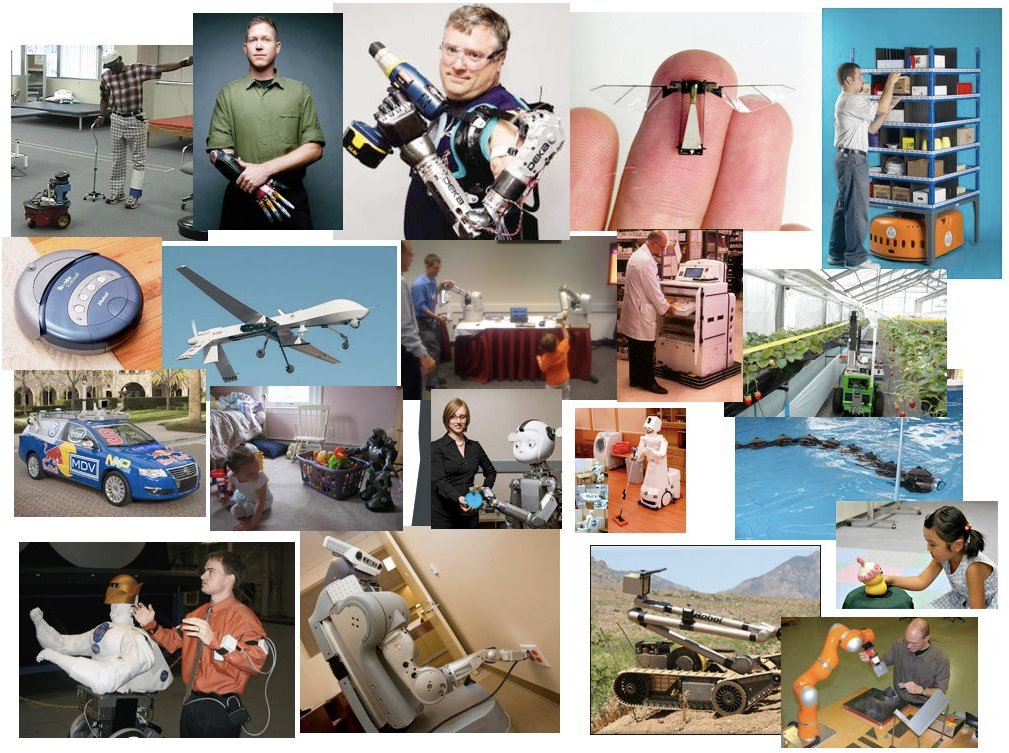
\includegraphics[width=0.7\textwidth]{figures/1_robotic_applications.jpg}
\caption{Examples of robotic applications.}
\label{fig:1_robotic_applications}
\end{figure}

Given this wide array of applications, it is important to note that robotics is not necessarily about to replace human labor.  Although not currently the case, at some point, robots may outperform humans at certain jobs due to being cheaper, faster, or easier to train.  However, robots will not and should not be the right solution for all of society's labor.  Rather, robotics should complement human productivity. There are many tasks that will remain difficult for robots, such as those that involve intuition, uncertainty, or human sociability.  The most productive use of robots will likely specialize robotic tasks to those that are not necessarily suited to or desired by their human users.  For example, instead of spending an hour vacuuming their house, a human user can delegate this task to a robot and spend this hour exercising.

\begin{figure}[!h]
\centering
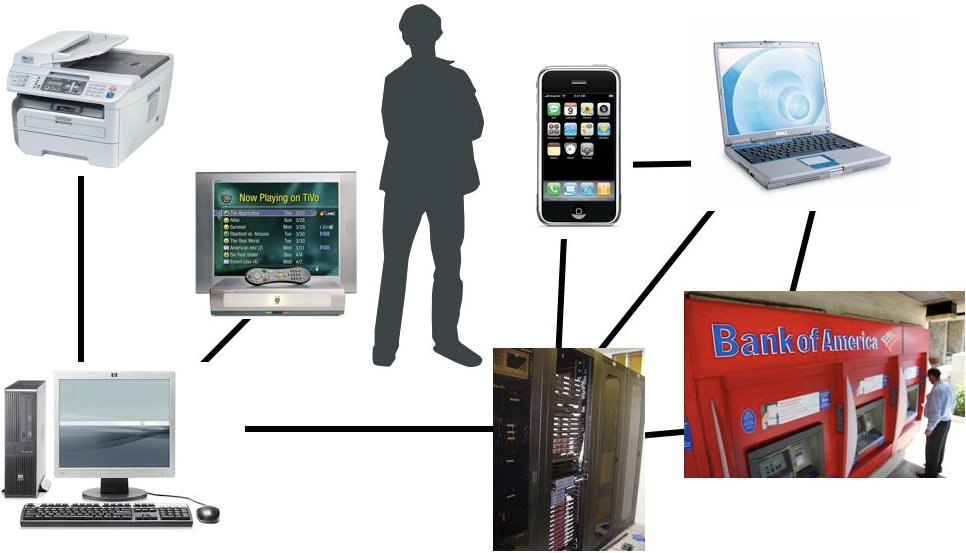
\includegraphics[width=0.7\textwidth]{figures/1_personal_computing.jpg}
\caption{Examples of heterogeneous computing devices.}
\label{fig:1_personal_computing}
\end{figure}

%\cjenkins{add note about many heterogenous devices for a single individual}

Robotics can also be thought of as an extension of computing and the Internet beyond digital worlds into the physical world that we inhabit. The explosion of personal computing devices present in our everyday lives, as seen in Figure \ref{fig:1_personal_computing}, have become not just an amenity but a necessity. Personal computing has enabled individuals to significantly increase their productivity in digital domains, such as electronic communication, publishing, and virtual telepresence (teleconferencing, video games, etc.).  Similarly, the prevalence of commodity robotic devices will move this productivity past the digital boundary and into the physical world. 

\begin{figure}[!h]
\centering
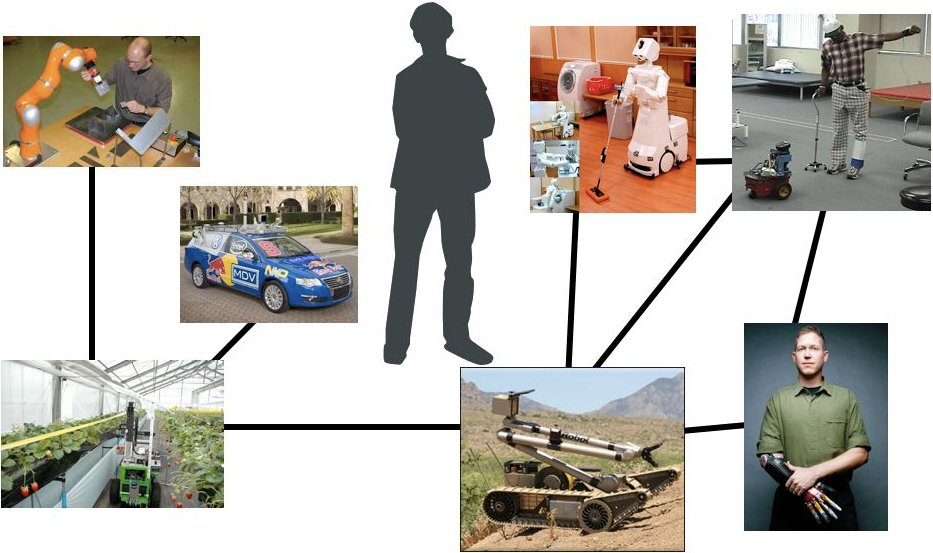
\includegraphics[width=0.7\textwidth]{figures/1_robot_apps.jpg}
\caption{Examples of heterogeneous robotic devices.}
\label{fig:1_robot_apps}
\end{figure}

Finally, whereas personal computing has enabled individuals to manage digital information by supervising teams of heterogeneous computing devices, autonomous robotics will enable individuals to manage physical environments by supervising teams of heterogeneous robotic devices, as seen in Figure \ref{fig:1_robot_apps}. If a heterogeneous collection of robots is to affect the physical world by interacting with and manipulating its features to achieve a predefined desire, the coordination among the robotic devices is essential. The question of how to coordinate and control a team of heterogeneous robotic devices is still an open challenge and needs to be addressed for this vision to be realized. 

\subsection{The Personal Robotics Revolution}

\begin{figure}[!h]
\centering
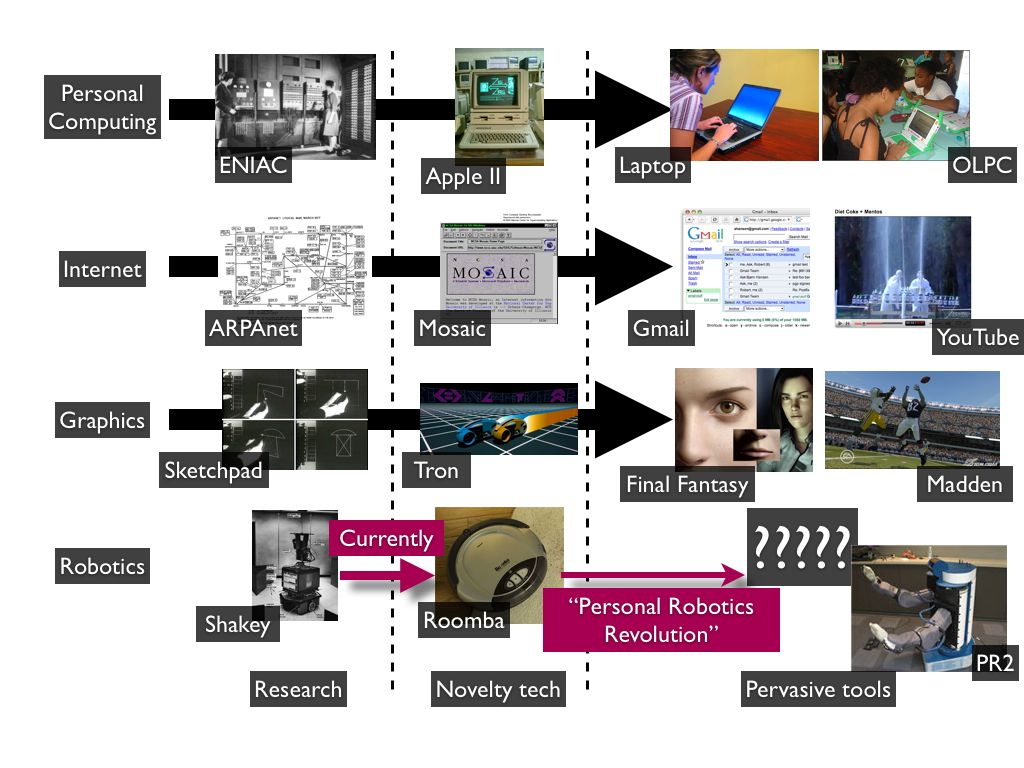
\includegraphics[width=0.85\textwidth]{figures/1_revolution.jpg}
\end{figure}

While problematic, the challenges of the physical world offer new and great opportunities for the pioneering spirit.  Think of robotics as a means to extend computing and the Internet beyond controlling digital environments into autonomously working in the physical world.  This is the perfect time to be a roboticist because innovators can shape the technology!  Similar to the ``personal computing revolution'' a few decades ago, robotics is on the dawn of its own \href{http://fora.tv/2009/05/30/Rodney\_Brooks\_Remaking\_Manufacturing\_With\_Robotics}{``personal robotics revolution''}, with many great robotic technologies that are now starting to come together. 

Robotics is currently in the same stage of the exponential technology growth as personal computing in the 1970s, computer graphics in the 1980s and the Internet in the early 1990s.  These three trends all hit the technology exponential, explained by Moore's law which describes ``a long-term trend in history of computing hardware, in which the number of transistors that can be placed inexpensively on an integrated circuit has doubled approximately every two years."\footnote{\href{http://en.wikipedia.org/wiki/Moore\%27s_law}{Moore's law: en.wikipedia.org/wiki/Moore\%27s\_law}}. Robotics is currently a technology exponential in the making, thus this is the time to get involved in robotics!

\subsection{CS 148 Disclaimer: the real world is unforgiving}

\begin{wrapfigure}{l}{0.35\columnwidth}
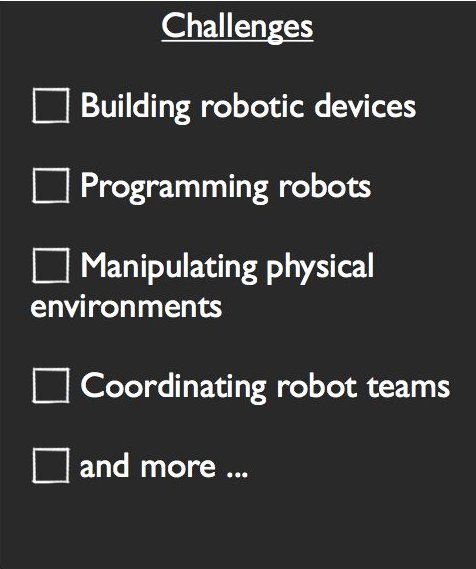
\includegraphics[width=0.3\columnwidth]{figures/1_challenges.jpg}
\end{wrapfigure}

The first prerequisite for building intelligent robots is to engineer robotic devices. Provided the abundance of robot systems along with the commercial availability of relatively cheap robots such as the Roomba, for the purposes of this class we will assume this prerequisite has been successfully met. The next challenge is to program robots to function autonomously in an unpredictable world. This is the challenge CS148 will address.

This course involves a significant amount of programming and decision making under uncertainty. Robotics is about understanding and functioning in the real world. However, the real world is highly dynamic, uncontrolled, and nondeterministic. These factors result in uncertainty that is unlike the structure and determinism of traditional computer science. Programming in the face of such uncertainty is a persistent challenge faced at all levels of robotics. Keep in mind that robots are not sentient, but their programmers are!


\section{Autonomous Robotics}

%Autonomy means an independence of control. In robotics this refers to the ability of a robot to perform desired tasks by making decisions and acting on them without any human intervention. 

We define an autonomous robot as a decision making agent with a physical embodiment that acts solely based on its perception of the world through sensors and its own internal information.  Teleoperated robots, or robots that are controlled by human operators, are not autonomous and are not studied in this course. Because humans are not directly making decisions for the robot, an autonomous control program must be executed that performs the ``cognitive'' functions of the robot, specifically: perception, decision making, and executing actions (or motion control). Combined these components act as the brains for the robot and enable the robot to be autonomous. 

CS148 is the study of autonomous robotics. That is, given robot hardware with sensing and actuation, we are challenged with programming the robot to autonomously perform a task. The algorithms and architectures for autonomous robot control are studied, which provide the ability to perceive, make decisions and act. It is important to note that this course is not a robotics engineering course. We will not build robot hardware, nor study in detail the physical dynamics and kinematics for expressing motion or robot control theory. CS148 utilizes a relatively cheap robot platform that allows us to study both in theory and in practice the core concepts of autonomous control.

\subsection{Robot Control Loop}

\begin{figure}[!h]
\centering
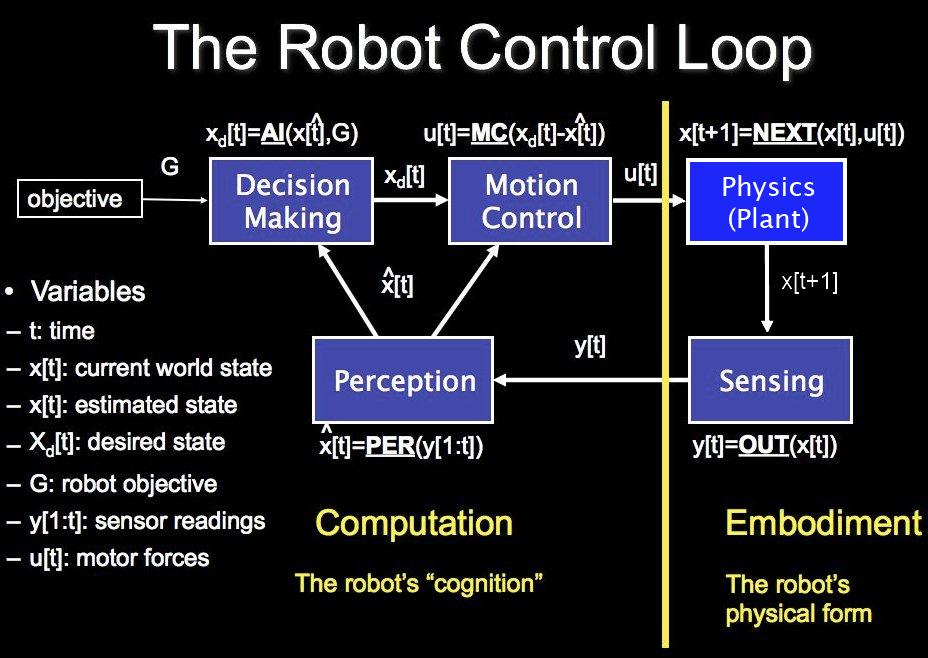
\includegraphics[width=0.85\textwidth]{figures/1_control_loop_white.png}
\label{fig:1_control_loop}
\end{figure}

The functions of all autonomous robots can be cast into a robot control loop. The robot control loop must be examined under the five main components that constitute an autonomous robot: plant, sensors, perception, decision making, and movement (or motion control.

The physical embodiment of the robot and its dynamics with the world is called the \textit{plant}.  The plant, or robot platform, allows a robot to exist in the physical world and interact with other physical objects in its environment. The plant is the physical embodiment and is subject to the same laws of physics that apply to humans and any other object. The plant consists of the body of the robot, including motors and actuators; it is the material structure that is the robot's presence in the world.

The robot's \textit{sensing} is its observations about the current state of the world. The information the robot collects through its sensors serves as input for perceiving the environment's state.  Sensing does not provide a complete view of the world, but is rather partial observations from the robot's perspective.  
%The sensors are not to be confused with sensing; sensors are the hardware on the plant that actually receives data whereas sensing is the process of collecting information about itself and the current state of the world.

The \textit{perception} component of the control loop uses the readings gathered from sensing and perceives the information in terms of itself and the environment to estimate, to the best of its abilities, the current state of the world.

Because we would like to have our robots perform some function, every robot must have an ``objective'' or goal. The overall goal of a robot may have different levels of abstraction and the overall goal may consist of many sub-goals; however only one objective can serve as the input to the control loop during a single iteration. An autonomous robot uses both the perceived state of the world and an object to guide the \textit{decision making} component of the control loop. Decision making determines the next action the robot should take.

Finally, in order to change the state of the physical embodiment, robots must have \textit{motion control}, based on perception and decision making that dictates the next state of the robot in terms of its physical parts. The motion control calculates the control forces that should be applied to the actuators in order for the robot to enact the desired action.

Together the plant and sensors compose the ``embodiment'' of the robot: the physical body and a mechanism of sensing to gather information about the environment. CS148 does not cover in substance topics within robot engineering for building the embodiment (actuators, sensors, physical parts) of a robot. For robots that are teleoperated or explicitly programmed to perform a specific task without ``thinking'', our discussion of the robot control loop can end here; our robot would just consist of the embodiment. 
%However, this course is really interested in exploring what makes a robot autonomous and how can we solve the next problem using autonomous robots. Thus 
In contrast, CS148 focuses on the autonomous, or ``cognitive'', aspects of this loop, pertaining to programming procedures for perception (state estimation), decision making (deciding how to act), and motion control (executing decided actions).

Lectures and activities in CS148 are centered around the basic notion of an autonomous robot control loop, as illustrated in Figure \ref{fig:1_control_loop}. The algorithms that we study are cast as components in this loop that will be used to form complete project implementations. 

\section{Course Format}

Topics covered during lectures will be grounded implementations during interactive sessions and 7 assignments.  Interactive sessions are devoted to a hands-on introduction to Player/Stage/Gazebo, ROS, Matlab, and working with our iRobot Create platforms leading up to the projects.

\subsection{Assignments}

The first three assignments are introductions to basic issues defining autonomous robotics and implementing robot controllers using either the Player or ROS robot middleware:

\begin{figure*}
\centerline{
\mbox{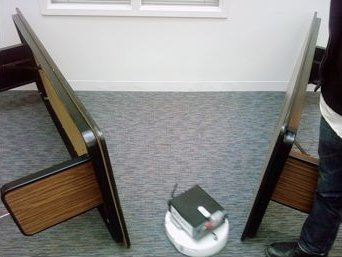
\includegraphics[width=2.01in]{figures/1_enclosure.jpg}}
\mbox{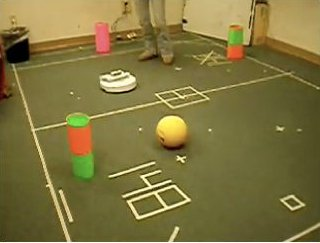
\includegraphics[width=1.99in]{figures/1_objrec.jpg}}
\mbox{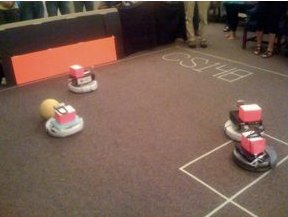
\includegraphics[width=2.0in]{figures/1_multi.jpg}}
}
\caption{Projects: Enclosure Escape, Object Recognition and Multi-robot Coordination.}
\end{figure*}

\begin{itemize}
\item Ch \ref{sec:create_spotting} Create Spotting: run experiments and analyze two built-in behaviors on the iRobot Create bases.
\item Ch \ref{sec:enclosure_escape} Enclosure Escape: implement a reactive random traversal robot control policy to escape from an enclosure.
\item Ch \ref{sec:object_seeking} Object Seeking: implement a control policy to continually seek and visit two objects in alternation.
\end{itemize}

The remaining projects explore different approaches to autonomous robot control in the context of robot soccer with various constraints on sensing and using heterogeneous robot hardware:

\begin{figure}[!h]
\centering
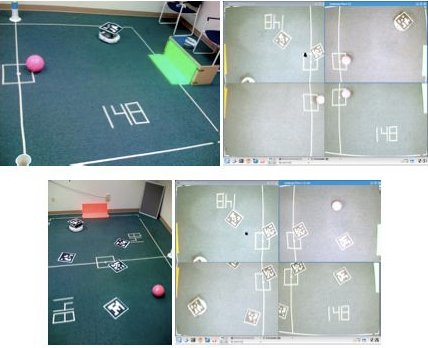
\includegraphics[width=0.6\textwidth]{figures/1_planning.jpg}
\caption{Path Planning Project.}
\end{figure}

\begin{itemize}
\item Ch \ref{sec:path_planning} Path Planning: given a map of the field and an overhead camera view of the environment, develop a deliberative planning-based robot client for visiting specific locations and pushing a ball into a goal.
\item Ch \ref{sec:localization} Monte Carlo Localization (MCL): same objective as path planning, except the camera view is onboard the moving robot.
\item Ch \ref{sec:subsumption} Subsumption: develop a goal scoring controller without maintaining any state (history or timing variables).
\item Ch \ref{sec:multi_robot} Multi-Robot Coordination: given a team of one SmURV/Create and one unknown robot platform, develop a competitive multi-robot strategy and individual controllers.
\item Ch \ref{sec:learning}  Learning: guide a fixed learning algorithm to play a control policy without explicit programming.
\end{itemize}

\subsection{Robot Soccer}

The CS148 projects all center around developing controllers to play robot soccer.  Robot soccer has been an active topic of research for over a decade.  RoboCup is the worldwide effort to advance the state of the art in robot soccer through yearly competitions.  Their goal is to field a team of robot soccer players capable of winning against the human World Cup champion by 2050 (Kitano).

\begin{figure*}
\centerline{
\mbox{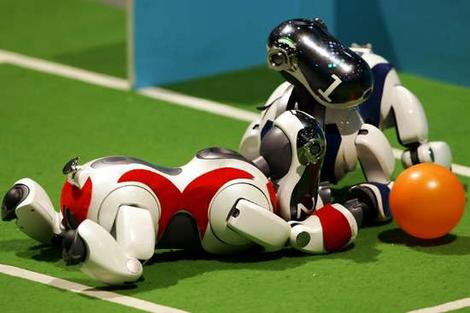
\includegraphics[width=2.98in]{figures/1_robocup06.jpg}}
\mbox{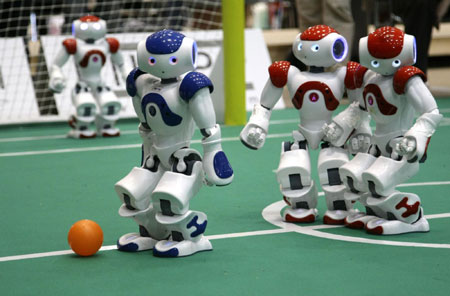
\includegraphics[width=3.00in]{figures/1_robocup09.jpg}}
}
\caption{4-legged League (RoboCup 2006); Standard Platform League (RoboCup 2009).}
\end{figure*}

This class considers a constrained version of this problem using the low-cost Brown iRobot Create platform and a highly structured soccer environment.  The robots programmed for the course projects will likely not outplay any humans or RoboCup-level robots, but provide a fun way to explore the basic topics in autonomous robot control.

\begin{figure*}
\centerline{
\mbox{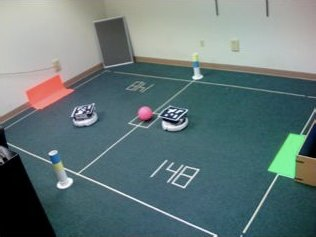
\includegraphics[width=3.04in]{figures/1_soccer1.jpg}}
\mbox{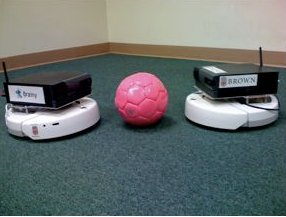
\includegraphics[width=3.00in]{figures/1_soccer2.jpg}}
}
\caption{Create platform robot soccer.}
\end{figure*}

\section{Project Deliverables}

Projects are graded assignments that consist of an implementation and a writeup.  Projects are to be implemented by student teams with individually composed written reports.  Implementations are demonstrated during scheduled class periods for grading by the course staff.  Project writeups are meant to explain student's work for the project with respect to the scientific method.  Due to the nature of robotics and programming in a nondeterministic world that is full of uncertainty, students will undoubtedly face many challenges implementing the projects. Given these challenges, experimentation and writing is essential for validating student's work.

\subsection{Project Writeups}

The purpose of the written reports is to familiarize the students with scientific writing and they should be written according to the scientific method.  The students must propose a central hypothesis, design experiments based on measurable evidence to test the hypothesis, and confirm the validity or invalidity of the hypothesis based on what was observed.  In this regard, they are not necessarily writing the document for themselves or the course staff, but rather to inform someone who is new to their work or the general topic.  Science is about general knowledge that is valid without being specific to a given time, place, or technology fads.

\section{How to use this book}

This book should be used as a hands-on guide to grounding concepts contained in the robotics textbooks (listed below) into implementable course modules.  Figure \ref{fig:1_venn} illustrates a Venn categorization of 
robotics textbooks into, ``Intro/Hobby'', ``Autonomous Robotics'', and ``Mechatronics''.  This book, as marked by the ``CS148" in Figure \ref{fig:1_venn}, is meant to combine the accessibility of an ``Intro/Hobby" (such as Martin's ``Robotic Explorations'' or Mataric's ``Robotics Primer'') with the concepts of an ``Autonomous Robotics" textbook (such as ``Principles of Robot Motion'' by Thrun et al). 
%Our aim is for anyone using this book to have both a general exposure to many robotic concepts as well as a more technical understanding of these concepts. Furthermore we provide an in depth guide on how to build a robot up through how to implement multi-robot coordination, provided general programming experience.

\begin{figure}[!h]
\centering
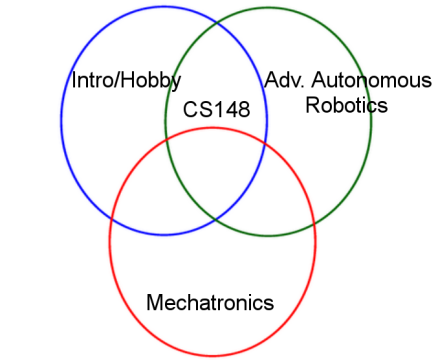
\includegraphics[width=0.5\textwidth]{figures/1_venn.png}
\caption{Types of robotic books and where CS148 falls within the spectrum.}
\label{fig:1_venn}
\end{figure}

\subsection{References}

\begin{itemize}
 
\item Matari\'c, \emph{The Robotics Primer}, MIT Press, 2007.
\item Wilson, \emph{How to Survive a Robot Uprising}, Bloomsbury USA, 2005.
\end{itemize}

\begin{wrapfigure}[10]{l}{0.15\columnwidth}
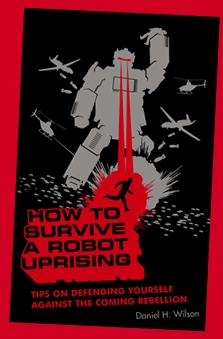
\includegraphics[height=0.25\columnwidth]{figures/1_robot_uprising.jpg}
\end{wrapfigure}

While Wilson's book has a humorous tone, it does cover many of the topics in CS148 in a substantive and accessible manner.  The other readings below are optional readings used in class.  Substantial material exists on web-accessible resources such as \href{http://wikipedia.org/}{Wikipedia} and the \href{http://www.aaai.org/aitopics/}{AI Topics Library} (specifically from the \href{http://www.aaai.org/aitopics/html/robots.html}{Robots} section).

\begin{itemize}
\item Siciliano and Khatib, \emph{Springer Handbook of Robotics}, Springer, 2008.
\item Arkin, \emph{Behavior-Based Robotics}, MIT Press, Boston, 1998.
\item Choset, Lynch, Hutchinson, Kantor, Burgard, Kavraki and Thrun, \emph{Principles of Robot Motion: Theory, Algorithms, and Implementations}, MIT Press, Boston, 2005.
\item Thrun, Burgard, and Fox: \emph{Probabilistic Robotics}, The MIT Press, 2005.
\item Martin: \emph{Robotic Explorations: A Hands-On Introduction to Engineering}, Prentice-Hall, 2001.
\item Spong, Hutchinson, and Vidyasagar, \emph{Robot Modeling and Control}, Wiley, 2005.
\item Craig: \emph{Introduction to Robotics: Mechanics and Control (3rd Edition)}, Addison-Wesley, 1989.
\item Bekey: \emph{Autonomous Robots: From Biological Inspiration to Implementation and Control}, The MIT Press, 2005.
\end{itemize}

\newpage
